\subsection{InceptionNet}
\begin{frame}{}
    \LARGE CNN Architectures: \textbf{InceptionNet}
\end{frame}

% InceptionNet
\begin{frame}[allowframebreaks]{InceptionNet}
    \begin{itemize}
        \item InceptionNet goes \textbf{deeper} with 22 layers.
        \item It is much more \textbf{efficient}: only 5 million parameters.
        \item Uses a special building block called the \textbf{Inception module}.
        \item Adds \textbf{1x1 convolutions} (bottleneck layers) to make the network faster and smarter.
    \end{itemize}

    \begin{figure}
        \centering
        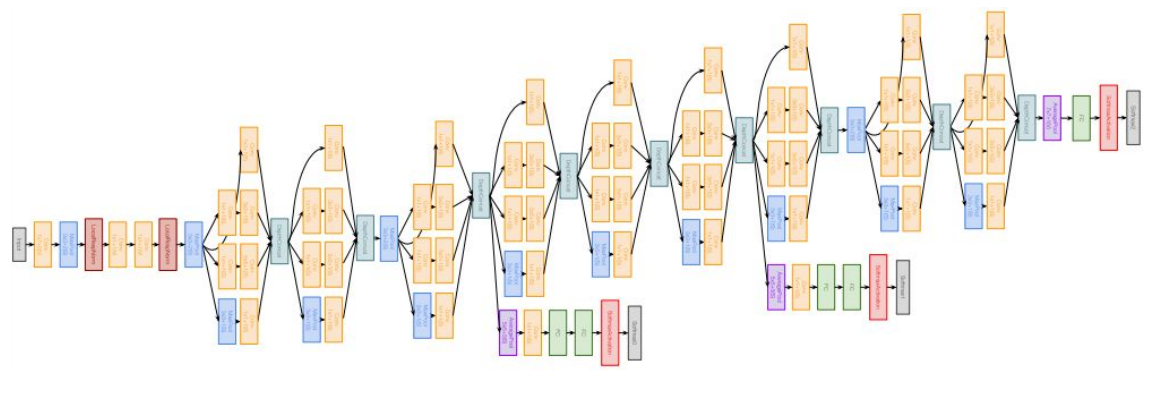
\includegraphics[width=1.0\textwidth,height=0.5\textheight,keepaspectratio]{images/cnn/inceptionnet_1.png}
    \end{figure}

\framebreak

    \begin{figure}
        \centering
        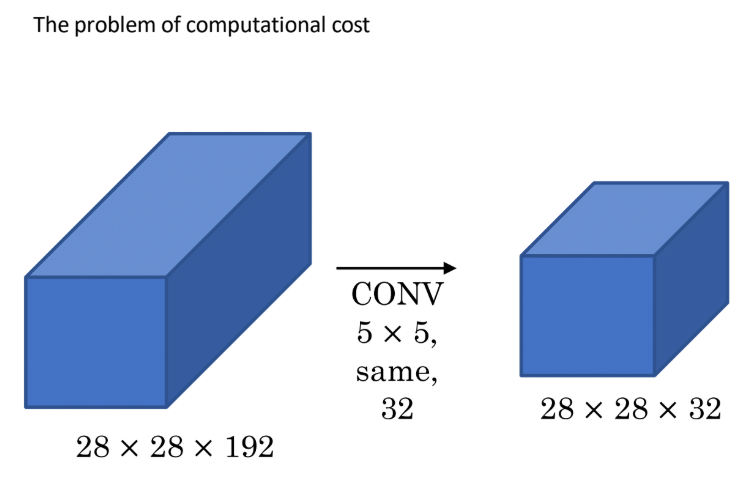
\includegraphics[width=1.0\textwidth,height=0.8\textheight,keepaspectratio]{images/cnn/inception-prob-1.png}
    \end{figure}

\framebreak

    \begin{figure}
        \centering
        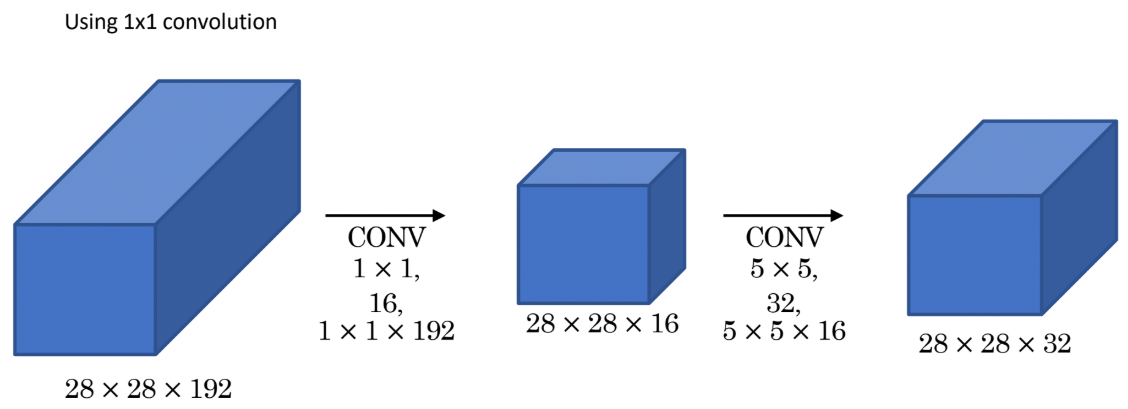
\includegraphics[width=1.0\textwidth,height=0.8\textheight,keepaspectratio]{images/cnn/inception-sol-1.png}
    \end{figure}

\framebreak

    \begin{itemize}
        \item \textbf{Inception module:} Uses multiple filter sizes ($1\times1$, $3\times3$, $5\times5$), in parallel, to capture different features, then combines their outputs.
    \end{itemize}

    \begin{figure}
        \centering
        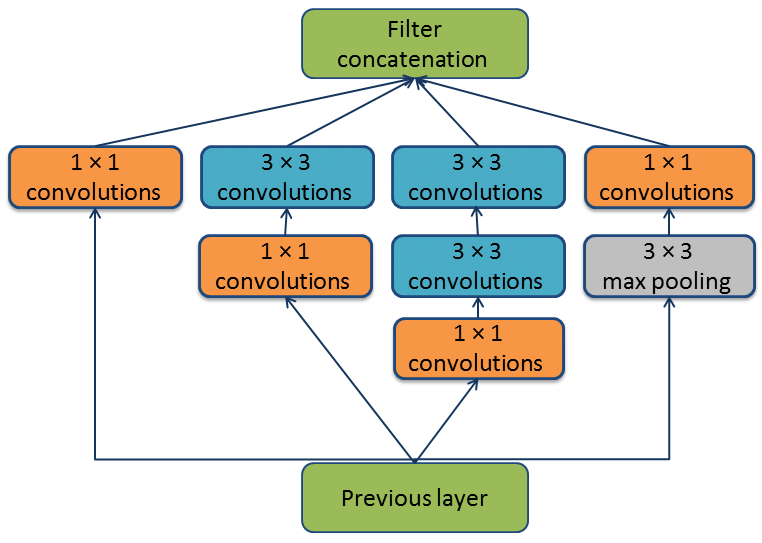
\includegraphics[width=1.0\textwidth,height=0.8\textheight,keepaspectratio]{images/cnn/inception_mod.png}
    \end{figure}

\framebreak

    \begin{figure}
        \centering
        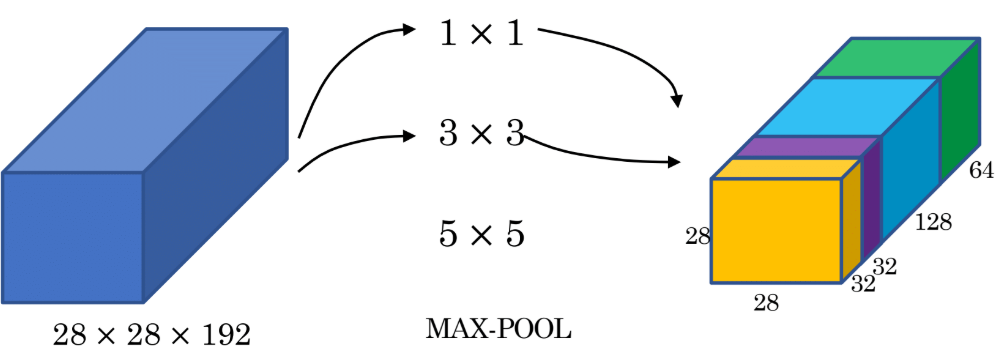
\includegraphics[width=1.0\textwidth,height=0.8\textheight,keepaspectratio]{images/cnn/inception-block.png}
    \end{figure}
    \vspace{2em}
    [Szegedy et al. 2014. Going deeper with convolutions]
\end{frame}